% Working manuscript, evaluation explanation revised 2026-10-23.
% Keep the user-approved original title; change only on explicit user request.
% All manuscript text, tables, and the TikZ diagram are embedded in this file.
% ASIACCS 2027: standard ACM two-column layout, no font/margin overrides.
% DOI, ISBN, submission ID and anonymous artifact URL remain unassigned.
\documentclass[sigconf,anonymous,pbalance]{acmart}
\usepackage{amsmath}
\usepackage{booktabs}
\usepackage{siunitx}
\usepackage{tikz}
\usetikzlibrary{arrows.meta,positioning}
\sisetup{group-separator={,},group-minimum-digits=4,group-digits=integer,detect-all}
\setcopyright{acmlicensed}
\copyrightyear{2027}
\acmYear{2027}
\acmDOI{}
\acmISBN{}
\acmConference[ASIACCS '27]{ACM Asia Conference on Computer and Communications Security}{July 12--16, 2027}{Macau}
\newcommand{\globalidx}{\mathrm{G}}
\newcommand{\ctx}{\mathcal{C}}

\begin{document}
\title{TAILGUARD: An Uncertainty-Driven Ensemble
Against Long-Tailed Cyber Threats}
\author{Anonymous}

\begin{abstract}
Intrusion detection systems faced the problem of incorporating sparsely labelled attacks without losing discrimination of benign traffic and previously labelled attacks.
Extreme gradient boosting (XGBoost) provided a strong baseline for tabular flow records, while a tabular prior-data fitted network (TabPFN) offered prediction conditioned on labelled examples through in-context learning.
We investigate TAILGUARD, a context-expert design that shares a frozen TabPFN backbone and separates expert activation from prediction adoption.
To establish the requirements for this design, we specify a single-model evaluation that separates classification under limited label availability from adaptation during sequential label release.
Each benchmark supplies its own training and evaluation records, and matched XGBoost and TabPFN comparisons use the same released examples and retention policies.
This protocol-focused draft distinguishes completed exploratory studies from proposed extensions and defines attack-wise quality, benign false alarms, retention, and computational cost without asserting an unverified performance or cost advantage.
\end{abstract}

\begin{CCSXML}
<ccs2012>
 <concept>
  <concept_id>10002978.10003001.10003002</concept_id>
  <concept_desc>Security and privacy~Intrusion detection systems</concept_desc>
  <concept_significance>500</concept_significance>
 </concept>
 <concept>
  <concept_id>10010147.10010257.10010258.10010259</concept_id>
  <concept_desc>Computing methodologies~Supervised learning by classification</concept_desc>
  <concept_significance>300</concept_significance>
 </concept>
</ccs2012>
\end{CCSXML}
\ccsdesc[500]{Security and privacy~Intrusion detection systems}
\ccsdesc[300]{Computing methodologies~Supervised learning by classification}
\keywords{intrusion detection, long-tailed classification, tabular foundation models, in-context learning, selective expert activation}
\maketitle

\noindent\textit{Protocol review draft, 23 October 2026.} The single-model evaluation establishes requirements for the context-expert design. Completed exploratory studies and proposed extensions are identified separately; historical result tables are omitted from this sharing version.

\section{Introduction}
\label{sec:intro}
Newly labelled attacks create a practical question for an intrusion detection system (IDS): how should the detector incorporate these examples without unnecessarily disrupting decisions on benign traffic and previously observed attacks? A classifier trained once on all available attack labels does not directly evaluate this update process. The issue is particularly relevant when attack classes have very different frequencies. Improving an average score can leave rare attacks undetected or increase the number of benign flows incorrectly labelled as attacks.

Our inputs are tabular flow records. We use extreme gradient boosting (XGBoost) as a strong supervised baseline~\cite{chen2016xgboost}. A tabular prior-data fitted network (TabPFN) offers a different mechanism: a pretrained predictor conditions on a labelled context~\cite{hollmann2023tabpfn,hollmann2025tabpfn}. With a frozen backbone, replacing or extending that context changes the prediction task without optimizing the backbone on each target dataset. The operational question is whether this mechanism yields useful attack detection and retention at an acceptable update and inference cost. The absence of backbone retraining alone is insufficient evidence of such an advantage.

Our research goal is to improve detection of under-represented attacks through the use of available labelled examples. Context composition is central to this goal because the examples presented to the predictor may be a limited subset of a much larger training pool. A single Global context must represent benign traffic and multiple attack families simultaneously. Additional contexts can emphasize Global error patterns, but emphasizing an attack may also cause an expert to predict it for benign flows or other attacks. Expert specialization therefore needs both a construction rule and a mechanism for deciding when its output is useful.

TAILGUARD investigates this combination. The current implementation constructs context experts from a shared anchor and residual-based blocks, using one frozen TabPFN backbone. A scorer evaluates candidate experts before expert inference; a verifier then assesses the selected expert's prediction before replacing the Global output. Expert construction, activation, and output adoption are separate decisions. We describe the implemented configuration without assuming that its present context recipe or selection objectives are final.

Label availability and retention capacity define different constraints. An attack-only preliminary study tests whether very few labelled examples can support attack-family discrimination before introducing benign competition or sequential updates. A subsequent comparison retains benign and previously labelled attacks while supplying examples of additional attacks from the same benchmark's training split. The current labelled set is therefore a subset of one source benchmark, not a second external dataset or a mixture of CIC2018 and ToN-IoT. The evaluation distinguishes which labels are available from when they become available and how many records are retained.

Two complementary evaluation views make these constraints explicit. LotBoNC's separation of known and novel classes informs the construction of label-availability conditions, although its unlabelled novel-class discovery task differed from our supervised adaptation task~\cite{hu2026lotbonc}. The stream study by Verma et al. informs prediction-before-label-release and separate accounting of memory maintenance and context processing~\cite{verma2026rethinking}. Our proposed extension uses these principles in a controlled label-release replay, without claiming that a class-introduction schedule reproduces the original traffic timeline. Both views compare a single TabPFN with XGBoost; extending the evaluation to the full expert bank remains a subsequent requirement.

Our contributions concern the design of TAILGUARD and the evidence needed to assess its use in long-tailed intrusion detection:
\begin{itemize}
\item \textbf{Residual-guided specialization through context.}
We construct a bank of experts by combining a shared labelled anchor with blocks selected from clusters of Global residual information. Specialization changes the evidence supplied to one frozen TabPFN backbone, rather than training separate expert weights. This connects expert construction to the reference detector's error patterns while retaining shared class coverage, instead of assigning each expert an exclusive attack class.
\item \textbf{Separate decisions to invoke an expert and adopt its output.}
We learn a pre-inference scorer for potential corrective value and a post-inference verifier for prediction adoption, using a separate route-training pool. Their combination makes specialization conditional on its estimated benefit over a retained Global decision: selecting an expert does not commit the system to replacing Global. The proposed contribution is this decision structure for residual-guided context experts, rather than expert routing alone.
\item \textbf{Explicit label, retention, and update budgets.}
We define a source-traceable evaluation with matched labelled rows for XGBoost and TabPFN. One view isolates classification with few newly labelled attacks, while a second follows successive label releases and tracks previously introduced attacks. Retained record counts, benign false alarms, and update and inference costs qualify aggregate F1. This is an evaluation design and a basis for subsequent expert-system testing, not a claim that the proposed extensions have already demonstrated an advantage.
\end{itemize}
The implemented expert structure and explicit evaluation design are the scope of this draft; consistent tail gains and an operational cost advantage remain hypotheses to be tested.

\section{Related Work}
\label{sec:related}
We organize related work around task-specific tabular learning, tabular foundation models, context and posterior adaptation, and expert specialization.

\subsection{Task-Specific Tabular Learning}
XGBoost~\cite{chen2016xgboost} constructed a supervised tree ensemble through gradient boosting. In our study it represents a detector whose fitted parameters are updated from the available labelled examples. Earlier exploratory comparisons included both a matched training-subset baseline and a full-training-pool baseline. The proposed protocol matches the released examples to isolate label availability and updating.

\paragraph{Discussion.}
A static tree-model result does not by itself answer how the model behaves when the set of available attack labels expands. Our response is to compare explicit update procedures on identical cumulative examples and to investigate context changes as an alternative way of incorporating information. The chosen comparator is full XGBoost refitting; this is an experimental choice, not a claim that all tree-based updates require full retraining. New-attack performance, existing-class retention, benign false alarms, and both update and inference time must support any advantage attributed to context-based updating.

\subsection{Tabular Foundation Models}
TabPFN learned a prediction procedure through pretraining on synthetic tabular tasks and applied it to new datasets using in-context learning~\cite{hollmann2023tabpfn}. Subsequent work demonstrated strong performance on small tabular datasets and developed a more capable tabular foundation model~\cite{hollmann2025tabpfn}. These studies motivate using a pretrained predictor as a reusable component. Section~\ref{sec:tabpfn} defines the interface needed here, while checkpoint and implementation versions remain in the experiment metadata rather than serving as manuscript condition names.

\paragraph{Discussion.}
Strong general tabular performance does not determine which labelled examples should represent an imbalanced IDS dataset, nor whether changing that representation improves rare-attack detection without increasing false alarms. We investigate a Global context together with specialized contexts instead of assuming that one context is adequate for every query. The relevant evidence is the gain of the complete context-and-selection system over the same Global predictor, including cases where specialization introduces new errors. This is a problem addressed by our design, not a guarantee supplied by pretraining.

\subsection{Context and Posterior Adaptation}
\paragraph{BoostPFN}
BoostPFN~\cite{wang2025boostpfn} treated PFNs as weak learners to extend their use to larger datasets through boosting. It is a direct comparison for exploiting a training pool through multiple smaller PFN contexts rather than placing the entire pool in one model input.

\paragraph{LoCalPFN}
LoCalPFN~\cite{thomas2024retrieval} combined nearest-neighbour context retrieval with task-specific fine-tuning. It adapted the predictor to local subsets and directly addressed the limitations of a single context for larger and more complex tabular tasks. The earlier exploratory LoCalPFN comparison included its fine-tuning stage.

\paragraph{DistPFN}
DistPFN~\cite{lee2026distpfn} adjusted test-time class probabilities using the context class prior and aggregated model predictions to address label shift, without additional model training. The earlier exploratory comparison applied its posterior adjustment to stored Global TabPFN-v3 probabilities while retaining the Global context.

\paragraph{Discussion.}
These methods address complementary adaptation problems: BoostPFN builds an aggregate predictor through boosting, LoCalPFN combines local context retrieval with fine-tuning, and DistPFN corrects posterior class-prior effects. For our IDS objective, the remaining question is when a specialized prediction should replace an existing Global decision, especially if gaining recall on an attack also creates false positives on benign traffic or other attacks. TAILGUARD investigates a reusable residual-guided context bank with a frozen backbone and separate invocation and adoption decisions. Its contexts provide candidate corrections, while the selection policy estimates their value relative to Global. This mechanism must be assessed through attack-wise precision and recall, corrections and new errors, and measured cost. 

Comparisons must also disclose differing information access and adaptation work, including LoCalPFN's fine-tuning and DistPFN's use of aggregate unlabelled test predictions. Their different objectives alone do not establish an IDS performance limitation or a TAILGUARD advantage.

% REF-ADDED 2026-10-23: task boundaries verified against the provided originals.
\subsection{Novel Classes and Sequential Evaluation}
LotBoNC~\cite{hu2026lotbonc} studied long-tailed botnet traffic with labelled known classes and an unlabelled mixture of known and novel classes. Its method used traffic representations, constrained pseudo-label assignments, and iterative prototype and prior updates to discover novel groups. The evaluation controlled which class labels were available and the composition of the unlabelled mixture. It did not specify the prediction-before-update stream protocol used in our second evaluation view.

\paragraph{Discussion.}
LotBoNC provides a useful precedent for explaining how one benchmark supplies deliberately constructed information conditions. Our comparison instead supplies a positive number of labels for each attack to be classified by name. XGBoost and frozen TabPFN are not treated as unlabelled novel-class discovery methods, and LotBoNC's clustering accuracy is not substituted for our class-wise F1. The proposed expert design must first show useful discrimination of these sparsely labelled classes under the same information budget; an unknown-class detector would require a separate mechanism and evaluation.

Rethinking Tabular Foundation Models On Data Streams~\cite{verma2026rethinking} evaluated predictions before labels became available and separated memory size, memory policy, label delay, and serving cost. The study found strong simple-memory baselines and substantial repeated context-processing costs. Its cache experiment concerned compact models and did not establish equivalent incremental updates for our TabPFN-v3 implementation.

\paragraph{Discussion.}
This stream protocol motivates explicit ordering of predictions, label release, and updates in our controlled replay. The proposed expert system would additionally need to account for expert-context construction and scorer/verifier updates, beyond the single-PFN costs measured first. A comparison with batch-refitted XGBoost addresses that specified baseline rather than all streaming learners. Claims about timestamp-faithful deployment or superiority over streaming methods require an appropriate temporal split and streaming baselines beyond the present comparison.

\subsection{Context Distillation}
In-context data distillation~\cite{ma2024icd} optimized synthetic context features while keeping the PFN weights and context labels fixed. Its experiments compressed information from a larger labelled training pool into a small retained context. The retained context size therefore differed from the amount of labelled information used during optimization.

\paragraph{Discussion.}
Distillation is a candidate for reducing context storage after labelled history becomes available. It does not by itself establish discrimination when only a few labels have ever been observed. A later TAILGUARD comparison must hold the accessible label history and total retained context budget fixed, count optimization and validation costs, and distinguish synthetic context features from original flow records. No distillation component is treated as validated by the two-model evaluation in this draft.

\subsection{Long-Tailed Expert Specialization}
\paragraph{Learning complementary experts.}
RIDE~\cite{wang2020long} combined multiple distribution-aware experts with a diversity objective and dynamic routing for long-tailed recognition. ACE~\cite{Cai_2021_ICCV} trained complementary experts on class subsets and used a distribution-adaptive optimizer to coordinate their learning. These approaches provide precedents for constructing diverse specialists under class imbalance; RIDE also makes conditional expert computation an existing part of this literature.

\paragraph{Discussion.}
RIDE and ACE learn specialization through expert parameters and training objectives. Our setting instead requires constructing specialized labelled contexts for a shared frozen predictor. TAILGUARD uses Global residual patterns to select specialty blocks and a common anchor to retain class coverage, so an expert need not own a disjoint class subset. The research question is whether this context-based specialization produces useful corrections without attracting false positives from other classes. We therefore evaluate experts on common populations and distinguish their predictions from the changes retained by the policy. This tests a different construction mechanism; it does not claim that learned experts or routing are themselves new, or that residual clustering guarantees useful specialization.

\paragraph{Expert aggregation.}
SADE~\cite{Zhang_2022} learned diverse experts for different class distributions and used self-supervised test-time aggregation when the test class distribution is unknown. BalPoE~\cite{Aimar_2023_CVPR} extended logit adjustment to a product of experts, with calibration supporting its balanced-error objective and mixup used to improve calibration. These methods show that how expert outputs are combined, and the distribution for which they are calibrated, are central to long-tailed recognition.

\paragraph{Discussion.}
SADE addresses adaptation of aggregation to an unknown test distribution, while BalPoE targets a balanced decision rule through calibrated expert combination. Neither objective alone determines whether invoking a particular context expert will improve a retained Global prediction. We address that decision with a scorer before expert inference and a verifier after inference, allowing the system to keep Global even after calling an expert. Evaluation must measure corrections and new errors together with attack-wise precision, recall, and benign false alarms. Calibration across contexts remains a validation requirement: the verifier is a learned decision rule, not a calibration guarantee. Our current experiments assess this intervention mechanism and do not establish superiority under unknown class priors or distribution shift.

\section{Preliminaries}
\label{sec:prelim}
\subsection{Long-Tailed Classification}
Let $\mathcal{D}=\{(x_i,y_i)\}_{i=1}^{N}$ contain tabular inputs $x_i\in\mathbb{R}^{d}$ and labels in $\mathcal{Y}=\{1,\ldots,C\}$. Class counts $n_c$ may differ substantially; the imbalance ratio is $\max_c n_c/\min_c n_c$ over nonempty classes. We use \emph{tail} descriptively for classes with small support in the fixed evaluation population and report that support explicitly. The number of examples selected into a context is a separate quantity. A rare class need not be difficult, and a difficult class need not be the rarest.

For each class, precision measures the correctness of predictions assigned to that class, while recall measures coverage of its true examples. F1 combines the two; macro-F1 gives equal weight to the included classes. A class can attain high recall by attracting many predictions and still have low F1 because of false positives. Benign false-alarm rate is the fraction of true benign examples predicted as attacks. These quantities must be interpreted together.

\subsection{TabPFN and In-Context Learning}
\label{sec:tabpfn}
A TabPFN prediction is conditioned on a labelled context $\ctx=\{(x_j,y_j)\}_{j=1}^{m}$ and an unlabelled query $x$~\cite{hollmann2023tabpfn,hollmann2025tabpfn}:
\begin{equation}
 p_{\theta}(y\mid x,\ctx),\qquad
 \hat y=\arg\max_{c\in\mathcal{Y}}p_{\theta}(c\mid x,\ctx).
 \label{eq:icl}
\end{equation}
In frozen-backbone use, $\theta$ is held fixed across target tasks. The labels in $\ctx$ belong to context examples; the query's true label is not supplied. Changing $\ctx$ changes the conditioning information even when $\theta$ is unchanged.
% REF-ADDED 2026-10-20: grinsztajn2026tabpfn3, Sections 2.3 and 2.4.2.
% Source: https://arxiv.org/html/2605.13986v2#S2.SS4.SSS2
% Supports preprocessing and context-dependent KV-cache work, not an IDS cost advantage.
Implementation work such as preprocessing and cache construction may still be required when a context is updated~\cite{grinsztajn2026tabpfn3}. Fine-tuning is a different mode of use and is stated explicitly when a baseline employs it.

\subsection{Experts and Conditional Computation}
An expert ensemble contains predictors $f_1,\ldots,f_K$ whose information or specialization may differ. Mixture-of-experts models use input-dependent mechanisms to select or combine expert outputs~\cite{jacobs1991adaptive}. Here we require only the general distinction between the expert bank and the rule for using that bank. An activation mechanism may select a subset of experts; an output decision may subsequently retain a reference prediction or use an expert prediction. Experts need not own disjoint classes, and activation does not necessarily imply adoption. The construction and decision rules specific to our system are introduced in Section~\ref{sec:approach}.

\section{Proposed Approach}
\label{sec:approach}
\subsection{Objective and Information Flow}
We seek corrections to a Global classifier that improve under-represented attack detection while controlling damage to existing decisions. Define $p_{\globalidx}(x)=p_{\theta}(\cdot\mid x,\ctx_0)$ and $p_k(x)=p_{\theta}(\cdot\mid x,\ctx_k)$ for the Global context and expert contexts. The Global and experts use the same pretrained backbone; specialization is implemented through their contexts. Separate lightweight models learn the scorer and verifier functions. Figure~\ref{fig:architecture} distinguishes their roles.

\begin{figure*}[t]
\centering
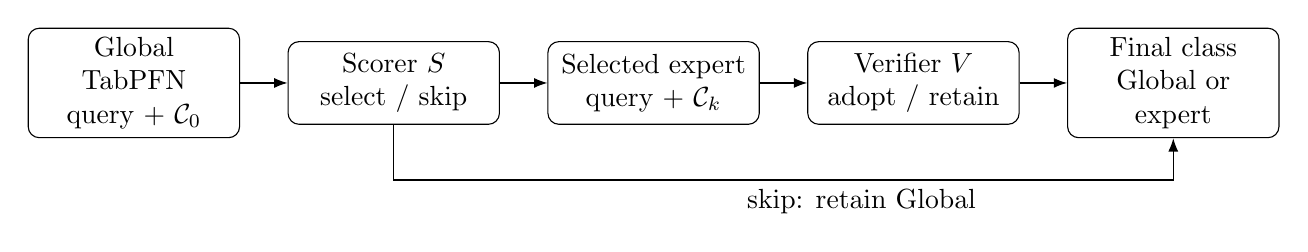
\begin{tikzpicture}[box/.style={draw,rounded corners,align=center,text width=2.45cm,minimum height=1.05cm},>=Latex]
\node[box] (g) at (0,0) {Global TabPFN\\query + $\ctx_0$};
\node[box] (s) at (3.3,0) {Scorer $S$\\select / skip};
\node[box] (e) at (6.6,0) {Selected expert\\query + $\ctx_k$};
\node[box] (v) at (9.9,0) {Verifier $V$\\adopt / retain};
\node[box] (o) at (13.2,0) {Final class\\Global or expert};
\draw[->] (g) -- (s);
\draw[->] (s) -- (e);
\draw[->] (e) -- (v);
\draw[->] (v) -- (o);
\draw[->] (s.south) -- ++(0,-.7) -| node[pos=.3,below]{skip: retain Global} (o.south);
\end{tikzpicture}
\caption{Query-time decisions in the current design. The context bank is constructed beforehand from training data. A scorer selects at most one expert; a verifier may retain the Global output even after that expert is called. The current experiments evaluate this policy using cached expert predictions, not a measured online conditional-inference service.}
\Description{A Global prediction is passed to a scorer. The scorer either skips expert inference and retains Global, or selects an expert. A verifier decides whether to adopt that expert's output or retain Global.}
\label{fig:architecture}
\end{figure*}

The static experiments partition the clean training data into Global-context, expert-construction, and route-training pools. Validation data are used for calibration and policy selection; test labels are used only for evaluation and explicitly identified diagnostics. The route pool is separate from the examples used to construct the Global and expert contexts. This separation prevents the scorer's training targets from simply reusing the experts' own context examples. It does not turn a repeatedly inspected development holdout into an untouched final evaluation set.

\subsection{Global Context and Residual-Based Experts}
The current Global context contains $100{,}000$ labelled examples. To construct specialists, we evaluate the Global model on the expert-construction pool. Its residual representation combines an input embedding, Global class probabilities, a signed error vector $\mathrm{onehot}(y)-p_{\globalidx}(x)$, and a class-balanced loss signal. The implementation normalizes these components and uses clipped loss weights in clustering. Thus, residual information describes errors of this particular Global model; it is not a direct observation of the true class boundary.

Weighted clustering produces $K$ groups. A diversity selection procedure extracts a block $B_k$ from each group, and each expert receives
\begin{equation}
 \ctx_k=A\cup B_k,\qquad k=1,\ldots,K,
 \label{eq:context}
\end{equation}
where $A$ is a common labelled anchor. Context construction includes correctly classified examples as well as errors; it is not an error-only filter. The current anchor covers all classes, so even a single-class specialty block does not make the complete expert a single-class classifier. Nevertheless, a large skewed block can dominate the expert's predictions, which motivates reporting context composition and false positives.

For the existing $K\in\{2,4,6,8\}$ sweep, the anchor contains $12{,}224$ CIC2018 examples or $18{,}717$ ToN-IoT examples. Each specialty block has an upper bound of $186{,}000$ examples and uses fewer when its cluster is smaller. Increasing $K$ therefore changes total stored context and repeated-anchor overhead. The sweep measures the behaviour of this construction rule, not expert count at a fixed total memory budget.

\subsection{Scoring Before Expert Inference}
The scorer estimates the value of invoking each expert using information available before obtaining that expert's prediction: Global outputs, an input representation, distance to the observable part of a cluster, and context descriptors. On the separate route pool, each expert is evaluated to construct the target
\begin{equation}
 d_k(x,y)=\mathbf{1}[\hat y_k=y]-\mathbf{1}[\hat y_{\globalidx}=y].
 \label{eq:decisiongain}
\end{equation}
This target is $+1$ for a correction, $-1$ for damage, and zero when correctness is unchanged. The present scorer uses class-balanced regression to estimate this quantity. It is a surrogate for useful intervention, not a direct optimizer of macro-F1. The highest-scoring expert is the candidate; a validation-selected threshold determines whether it is activated. A no-intervention policy is an explicit candidate during policy selection.

The expert outputs used to create training targets are available offline on already labelled route data. No query label or candidate-expert output is supplied to the scorer during evaluation. This offline training procedure should not be interpreted as requiring collection of future deployment errors to construct each new query's context.

\subsection{Verification and Output Adoption}
After candidate inference, the verifier uses both Global and expert probabilities, affinity features, and expert descriptors. Its current training target is the improvement in log probability of the true route-pool label,
\begin{equation}
 \ell_k(x,y)=\log p_k(y\mid x)-\log p_{\globalidx}(y\mid x).
\end{equation}
The implementation fits a lower-quantile regressor with quantile $0.25$. The verifier's score is a learned surrogate; it is neither a certified lower bound nor a guarantee that the expert's top class is correct. The system adopts the candidate only when both the activation and verification thresholds are passed. Otherwise it retains the Global prediction. Accepted outputs may equal Global outputs, so activation, acceptance, and label changes are counted separately.

Thresholds are selected on a validation subset to improve macro-F1 subject to limits on benign false alarms, selected protected classes, and a designated tail group. A separate validation confirmation subset is not used for threshold selection. The implemented false-alarm constraint permits at most $0.05$ percentage points of increase on the weighted selection population. This is a validation constraint, not a bound on future test behaviour. 

The current policy groups Bot, Infiltration, and Web attacks as the CIC2018 tail set, and MitM and Ransomware as the ToN-IoT tail set. Protected classes are Brute force, DDoS, and DoS for CIC2018, and DDoS and DoS for ToN-IoT. Validation weights reflect the clean training class proportions. These are existing policy settings, not a new universal definition of tail classes. Final choices of objectives, constraints, and context recipe remain open.

\subsection{Expert Diagnostics and the Oracle Distinction}
\label{sec:diagnostics}
We distinguish three questions. First, how does each expert classify the same evaluation population? Raw multiclass predictions and per-class precision, recall, and F1 include errors on all other classes. Second, which corrections survive the executable scorer/verifier policy? These are measured relative to Global on the same rows. 

Third, what happens under a label-assisted assignment based on the full residual representation? In this diagnostic, the true test label is used only to assign a sample to the closest residual cluster; the assigned expert still receives only its context and the unlabelled query.

We call the third procedure a \emph{residual-assignment oracle diagnostic}. It does not choose whichever expert happens to be correct, and it is not a guaranteed upper bound. Its assigned population differs from a label-free assignment based on observable features and Global probabilities. Consequently, differences between these two populations cannot by themselves establish that an expert has learned or failed to learn a class boundary. Independent expert capability is assessed using common evaluation populations, while deployment value is assessed using a label-free policy.

\section{Evaluation}
\label{sec:eval}
\subsection{Evaluation Scope and Evidence Status}
The evaluation first establishes the conditions under which labelled context is useful for intrusion detection. Completed exploratory studies include attack-only learning curves with five seeds and a separate stage-wise comparison with three seeds, including XGBoost fitted on the same retained rows as TabPFN. They used fixed, previously examined benchmark splits. The two-view protocol below is a proposed refinement; no new results are assigned to it in this draft. The historical expert-system and 100,000-row experiments use different information budgets and are not evidence for the proposed small-label protocol.

\subsection{Data Quality and Evaluation Populations}
% REF-ADDED 2026-10-20: original benchmark provenance, separate from NF-v3.
% cic2018official: https://www.unb.ca/cic/datasets/ids-2018.html
% moustafa_toniot_2021 (existing BibTeX entry): https://doi.org/10.1016/j.scs.2021.102994
% luay2025NetFlowDatasetsV3 remains the source for our 46-feature representation.
We use the NF-v3 representations of CIC2018~\cite{cic2018official} and ToN-IoT~\cite{moustafa_toniot_2021} with 46 features~\cite{luay2025NetFlowDatasetsV3}. An audit found identical model-input vectors with different family labels. For the current experiments, every row belonging to such a conflicting vector group is removed. Feature equality is checked after the documented float32 conversion and non-finite-value handling. Remaining rows retain their original train, validation, and test memberships; there is no re-splitting after removal. Identical-feature rows with the same label are preserved.

% BEGIN embedded table: quality
\begin{table}[t]
\centering
\caption{Offline conflict filtering. All rows of an identical-input group with inconsistent family labels are removed; retained rows keep their original split membership. Counts refer to full datasets and splits, not selected contexts.}
\label{tab:quality}
\begin{tabular}{@{}l *{2}{S[table-format=8.0]}@{}}
\toprule
Population & {CIC2018} & {ToN-IoT} \\
\midrule
Original rows & 20115529 & 27520260 \\
Removed rows & 5360112 & 16712972 \\
Retained rows & 14755417 & 10807288 \\
Retained train & 8666430 & 4669119 \\
Retained validation & 3046514 & 3866446 \\
Retained test & 3042473 & 2271723 \\
\bottomrule
\end{tabular}
\end{table}
% END embedded table: quality

This operation changes the evaluation population substantially (Table~\ref{tab:quality}). It removes contradictions in the chosen feature representation; it does not prove that the original labels are erroneous, or solve all ambiguities of intrusion detection. The audit uses labels across the benchmark, so it is an offline curation protocol rather than a deployment-time filter. Scores describe this filtered population and must not be compared directly with published results on unfiltered data. Same-label identical features can remain across splits, which motivates additional duplicate- and session-aware validation before deployment claims.

\subsection{From One Benchmark to the Current Labelled Set}
\label{sec:construction}
The current labelled set contains selected training records from one benchmark. Let $\mathcal D_b^{\mathrm{tr}}$, $\mathcal D_b^{\mathrm{val}}$, and $\mathcal D_b^{\mathrm{te}}$ denote the retained splits of benchmark $b$. We run the procedure independently for CIC2018 and ToN-IoT, preserving source row identifiers and benchmark membership. A controlled schedule reveals selected training records and labels; it does not generate flow-feature values or transfer attacks between benchmarks. The source benchmarks were themselves collected in experimental environments, so using their recorded rows does not establish an uncontrolled production-traffic evaluation.

The initial labelled set $L_0$ contains 750 benign records and 125 records from each of two initial attack classes. A release $R_t$ contains newly available labelled training records, and the labelled history and retained memory are
\begin{equation}
 L_t=L_{t-1}\cup R_t\subseteq\mathcal D_b^{\mathrm{tr}},\qquad
 M_t=\operatorname{Keep}_{B}(M_{t-1}\cup R_t).
\end{equation}
Accumulation uses $M_t=L_t$; bounded retention limits $|M_t|$ to $B$, initially 1,000 in the existing studies. Newly supplied records enter in full, with FIFO, random, or similarity-based deletion of existing records; the implemented policies retain at least one example of each represented class. XGBoost is refitted on $M_t$, and frozen TabPFN uses the same ordered rows as context and rebuilds the necessary preprocessing and caches. Extra stored archives, validation labels, or learned context values must be disclosed separately from the retained-row count.

The former term ``current dataset'' refers to $L_t$ or, under bounded retention, $M_t$. For example, selecting 100 DDoS records extends the CIC2018 initial set from 1,000 to 1,100 under accumulation. With a 1,000-row memory, these records instead replace 100 existing records. The value 100 was an illustrative label-availability condition, not a daily arrival count, an optimum, or a statistic estimated from deployment. Existing runs varied it over 5, 10, 20, 30, 50, and 100 per newly introduced attack. All evaluation records remain outside the update sets.

\subsection{Attack-Only Preliminary Study}
\label{sec:fewshot}
Attack-only learning curves test the prerequisite that a small labelled context can discriminate attack families at all. Each class supplies the same number of training records, with no benign training records, and both models receive identical nested subsets at each sample count. Evaluation uses the attack portion of the fixed test split, with six classes in CIC2018 and nine in ToN-IoT. The extended curves distinguish model differences from additional gains available at larger sample counts. This study does not measure benign rejection, retention under updates, or performance of the proposed expert system.

The supervised IDS evaluation restores benign records and unequal old/new label counts. Positive-label conditions avoid treating a classifier without an output class as an unknown-class discovery method. At the smallest budgets, actual XGBoost tree splits and sensitivity to prespecified small-sample settings must also be checked. The observed learning curves motivate a limited-label regime but do not select only conditions favourable to TabPFN or establish a universal saturation point.

\subsection{View 1: Classification under Limited Label Availability}
\label{sec:availability}
Label availability is varied independently of update order. The proposed comparison combines the same $L_0$ with $n\in\{2,5,10,20\}$ training records from each additional attack class and evaluates one fitted XGBoost and one frozen TabPFN on the fixed benchmark test. Subsets are nested across $n$, and both models use identical row identifiers and preprocessing information. This view first uses all available labelled rows, so memory deletion does not obscure the label-efficiency comparison. Bounded-memory policies are assessed in View 2 with the same observed label history for both models. The 100-row condition remains a historical reference rather than a presumed optimum.

Attack-wise F1, precision, recall, and benign false-alarm rate quantify the effect of competition with existing classes. We report macro averages separately for newly labelled attacks and previously labelled classes, deriving their F1 values from the common mixed evaluation population. Test class frequencies are held fixed while label counts change. LotBoNC informs the explicit known/novel composition and label-access distinction, but this view supplies labels for new classes and performs supervised classification rather than reproducing LotBoNC's unlabelled clustering task~\cite{hu2026lotbonc}.

\subsection{View 2: Adaptation during Sequential Label Release}
\label{sec:sequential-design}
Sequential label release measures the path to an adapted detector rather than only its final score. The proposed controlled replay uses the same source training pool and final label allocation as View 1. It retains the established class-introduction schedule but reveals nested batches so that each new attack has 2, then 5, 10, and 20 available labels before the next introduction. For CIC2018, the initial attacks are Brute force and DoS, followed by DDoS, Web attacks, Infiltration, and Bot. For ToN-IoT, the initial attacks are Scanning and DoS, followed by Injection/DDoS, Password, XSS, Ransomware/Backdoor, and MitM; jointly introduced classes follow the same per-class budgets.

Prediction precedes the release of an arriving training record's label, following the information-order principle of prequential evaluation~\cite{verma2026rethinking}. Labels are then released according to the common experimental schedule, and both methods update at the same checkpoints. A separate fixed test panel measures post-update performance on benign traffic and all introduced attacks; test labels are used only for evaluation and never enter $L_t$ or $M_t$. The pre-release predictions and post-update panel scores are distinct estimands and are not pooled. Before its first label is available, a new class has no fitted output category in these baselines, so the mechanically zero class-identification score is not evidence of a successful novelty-detection mechanism.

Retention follows every introduced attack through subsequent updates, extending the earlier initial-versus-final comparison of only the initial classes. We compare performance on fixed evaluation rows and explicitly state the competing class set. The main adaptation curves begin after positive labels are available and show quality against acquired labels and cumulative computation. A shared final allocation makes cumulative endpoint scores a consistency check, while intermediate scores expose the consequences of update timing and memory deletion. This is a controlled replay of label-availability events, not a reconstruction of the original packet timeline or an evaluation of an operational annotation policy.

\subsection{Fair Comparisons and Cost Boundaries}
\label{sec:protocol-cost}
Information access is matched before comparing model families. XGBoost and TabPFN receive the same selected records under each retention policy, and cumulative and bounded-memory results remain separate. XGBoost uses explicit refitting at shared release checkpoints; this choice is not a claim that all tree methods require full retraining. TabPFN-v3 retains frozen pretrained weights, and context refresh includes the preprocessing and cache work actually performed. Model settings, seed repetitions, label access for validation, and subset policies are fixed before a new held-out assessment.

Update cost includes record selection or deletion, preprocessing, and model fitting or context-cache construction. Initial preparation and query inference are measured separately, with query batch size, hardware, and concurrency reported. Total processing cost is also evaluated for a fixed number of queries per update, since lower update time alone can coexist with higher inference cost. Actual retained records and model/cache memory are reported as different resource quantities. Context distillation remains a later candidate whose optimization time and accessible training history must be charged to the same budgets~\cite{ma2024icd}.


\section{Discussion}
\label{sec:discussion}
\subsection{What the Present Evidence Supports}
The completed preliminary studies support examining supervised adaptation with few attack labels, rather than assuming that small contexts are incapable of useful classification. They do not establish a uniform TabPFN advantage, adequate detection of every rare attack, or a low-cost streaming system. The revised protocol separates label efficiency, retention, and computation so that similar aggregate scores still yield an interpretable comparison. A model modification becomes justified when a specific failure persists under matched information and retention budgets. The expert-bank architecture remains a candidate response whose added information and computation require separate evaluation.

\subsection{Design Priorities and Required Validation}
The next context comparisons should hold the available labelled pool and total context budget fixed while varying which examples occupy that budget. Candidate directions include broader benign coverage, synthetic tail examples, learned representations for context construction, and explicit context selection objectives. These are prospective design choices, not components validated by the present results. Selection must use training and validation data, and each proposal must be evaluated for both attack recall and erroneous attack predictions on other classes.

Once a useful context design is selected, ablations should separate the scorer's choice of expert from the verifier's adoption decision using the same bank and fitted outputs. The update study must then be extended to the complete system: rebuilding contexts and updating the scorer/verifier have costs that a single-TabPFN comparison omits. This progression tests whether the architecture provides a practical update mechanism and useful tail detection, rather than treating repeated improvements to a static macro-F1 as the sole objective.

\subsection{Limits of Generalization}
Previously inspected benchmark splits limit confirmatory conclusions even when sampling is repeated across seeds. Filtering conflicting vectors changes class prevalence and removes a substantial portion of each dataset; same-label feature overlap may remain across splits. Feature-disjoint diagnostics do not replace session-disjoint or temporal validation. The proposed replay controls which labels are released rather than reconstructing an observed deployment stream. XGBoost and TabPFN establish a focused comparison; broader claims about stream learning require streaming baselines and timestamp-faithful data preparation. Zero-label novelty discovery remains a separate task requiring an appropriate output mechanism and evaluation.

\section{Conclusion}
We investigate a TabPFN-based detector that specializes through labelled contexts and separates expert activation from output adoption. A source-traceable single-model protocol establishes the label-efficiency and retention requirements before attributing benefits to the ensemble. Its complementary views distinguish classification with limited labels from the process of incorporating those labels over successive updates. The next validation compares attack-wise quality, benign decisions, and measured processing cost under matched information budgets, then tests whether targeted context or selection changes address the observed failures.

\bibliographystyle{ACM-Reference-Format}
\bibliography{ref}

\appendix
\section{Open Science}
\label{app:open-science}
\textit{Submission preparation pending.} The experiments retain commands, source snapshots, checkpoint identities, split and context IDs, predictions, and cost logs. The manuscript source metadata links retained evidence and protocol revisions to their input files and hashes. An anonymous, reviewer-accessible artifact package and persistent URL have not yet been prepared; they must be supplied before submission. Third-party code, checkpoints, and datasets must be distributed or referenced according to their respective licences.

\section{Ethical Considerations}
The reported work is an offline analysis of existing research datasets and does not involve deploying attacks or monitoring a live network. Incorrect attack predictions can burden operators, while missed attacks can create false confidence. We therefore report benign false alarms and class-specific errors alongside aggregate performance. Removing conflicting feature vectors is an evaluation choice, not evidence that comparable ambiguity will disappear in deployment. Before releasing artifacts, dataset and checkpoint redistribution permissions and the contents of retained row identifiers and metadata must be checked; no such release is claimed in this draft.

\end{document}
